\section{Implementazione del Storage Covert Channel} 
%ICMP: The Good, the Bad, and the Ugly
%https://www.researchgate.net/publication/224349250_Implementation_of_an_ICMP-based_covert_channel_for_file_and_message_transfer 
%
In uno Storage Covert Channel, la risorsa condivisa sarà il pacchetto ICMP 
inviato e i dati saranno scritti nei suoi campi. Il destinatario, una volta 
ricevuto, potrà poi leggere i valori codificati al loro interno. 
Nelle Tabelle \ref{table:icmpv4:tipologie} e \ref{table:icmpv6:tipologie} 
sono indicati le tipologie di messaggi sfruttate. Le tabelle indicano anche 
quali campi sono stati utilizzati e quanti byte pesa un singolo pacchetto. 
%Inoltre è stato indicato anche quant'è il peso di un singolo pacchetto di quella tipologia. 
\vspace{2ex} \newline 
Tuttavia, nel caso di alcune tipologie (come i messaggi Echo Request/Reply), 
si avranno delle varianti sia nella quantità di dati esfiltrabili sia sulla 
quantità di byte che vengono trasmessi per singolo datagram.  
Ciò è dovuto alla presenza del campo \textit{data} che permette di inserire 
una quantità maggiore di dati. 
%Questo perchè il messaggio può trasportare un payload al suo interno. 
%Le varianti implicheranno quindi l'utliizzazione o meno di questo campo. 
%Nel caso lo si utilizzi il payload o conterrà 32 byte di informazione oppure 56 byte; 
%il primo caso verrà usato perchè è il valore di defualt usato nei sistemi Windows il secondo è invece il sistema usato nei sistemi Linux. 
%Anche il TTL varierà, il suo valore sarà 128 nei sistemi windows mentre 64 nei sistemi Linux. 
%\vspace{2ex} \newline 
%Altre varianti potranno essere presenti per qeulle tipologie che richiedono il pacchetto che ha causato l'errore (Redirect, Destination Unreachable). 
%In questi casi si potranno usare diverse tipologie di pacchetti purchè la loro lunghezza non superi i 28 bit. 
%Possibili alternative trovate sono con IP/ICMP e con TCP/IP con entrambe che permettono l'invio di due byte. 
\begin{longtable}{|c|c|c|}
    \hline 
    \textbf{Tipologia} & \textbf{Byte per pacchetto} & \textbf{Campi Utilizzati}  \\ %messaggi di errore
    \hline
    Destination Unreachable  & 20+8+21 & unused(4 bytes) \\ 
    &$\rightarrow$min 49 byte& header+64 bits (2bytes)\\ %messaggi di errore
    \hline 
    Time Exceeded  & 20+8+21 & unused(4 byte)\\ 
    &$\rightarrow$min 49 byte&header+64 bits(2 byte) \\ %messaggi di errore 
    \hline
    Parameter Problem  & 20+8+21 & pointer(1byte)\\ 
    &$\rightarrow$min 49 byte&unused(3byte)\\ 
    &&header+64 bits(2byte)  \\ %messaggi di errore
    \hline 
    Source Quench   & 20+8+21 & unused(4byte)\\ 
    &$\rightarrow$min 49 byte&header+64 bits(2byte) \\ %messaggi di errore
    \hline     
    Redirect Message & 20+8+21=min 49 byte & header+64 bits(2byte) \\ %messaggi di errore
    \hline 
    Echo Request/Reply & 20+8+32 & identifier(2byte)\\ 
    &$\rightarrow$min 60 byte&data($\geq32$) \\ %messaggi di informazione
    \hline 
    Timestamp Request/Reply & 20+8+12+32& identifier(2byte)\\ 
    &$\rightarrow$min 72 byte&timestamp(4byte*3)\\ 
    &&data($\geq32$) \\ %messaggi di informazione
    \hline 
    Information Request/Reply & 20+8=28 byte & identifier(2byte) \\ %messaggi di informazione
    \hline 
    %9 & 0 & CC  & Router Advertisement & Routers announce themselves to hosts. \\
    %\hline
    %10 & 0 & CC  & Router Solicitation & Hosts request router advertisements. \\
    %\hline 
    \caption{Tipologie di messaggi ICMPv4 usati} 
    \label{table:icmpv4:tipologie} 
\end{longtable} 
\vspace{2ex}
\begin{longtable}{|c|c|c|} 
    \hline 
    \textbf{Tipologia} & \textbf{Byte per pacchetto} & \textbf{Campi Sfruttatti}  \\
    \hline
    Destination Unreachable & 40+8+41 & unused(4 bytes)\\ 
    &$\rightarrow$min 89 byte&invoking packet(2bytes) \\ %messaggi di errore
    \hline 
    Time Exceeded & 40+8+41 & unused(4 bytes)\\ 
    &$\rightarrow$min 89 byte&invoking packet(2bytes) \\ %messaggi di errore
    \hline
    Parameter Problem & 40+8+41 & pointer(4byte)\\ 
    &$\rightarrow$min 89 byte&invoking packet(2byte) \\  %messaggi di errore
    \hline 
    Echo Request/Reply & 40+8+32 & identifier(2byte)\\ 
    &$\rightarrow$min 80 byte&data($\geq32$) \\ %messaggi di informazione
    \hline 
    Packet Too Big & 40+8+41 & mtu(4byte)\\ 
    &$\rightarrow$min 89 byte&invoking packet(2byte) \\  %messaggi di errore
    \hline 
    \caption{Tipologie di messaggi ICMPv6 usati} 
    \label{table:icmpv6:tipologie} 
\end{longtable} 
%\import{./icmp}{messaggi_errore}  
%\import{./icmp}{messaggi_informativi} 


\subsection{Inserimento dei dati nei campi usati} 
\subsubsection{Campo \textbf{unused}}
Dalle specifiche RFC (792 \cite{icmpv4_message_type} e 4434 \cite{icmpv6_message_type})
il campo deve essere 0. Quindi Scapy, quando manderà il pacchetto, lo 
invierà conforme allo standard e di conseguenza azzererà qualsiasi valore 
al suo interno (come mostra la Figura \ref{fig:covertStorage:sourcequench:errScapy}). 
\newline
\begin{minipage}{\textwidth}
    \centering
    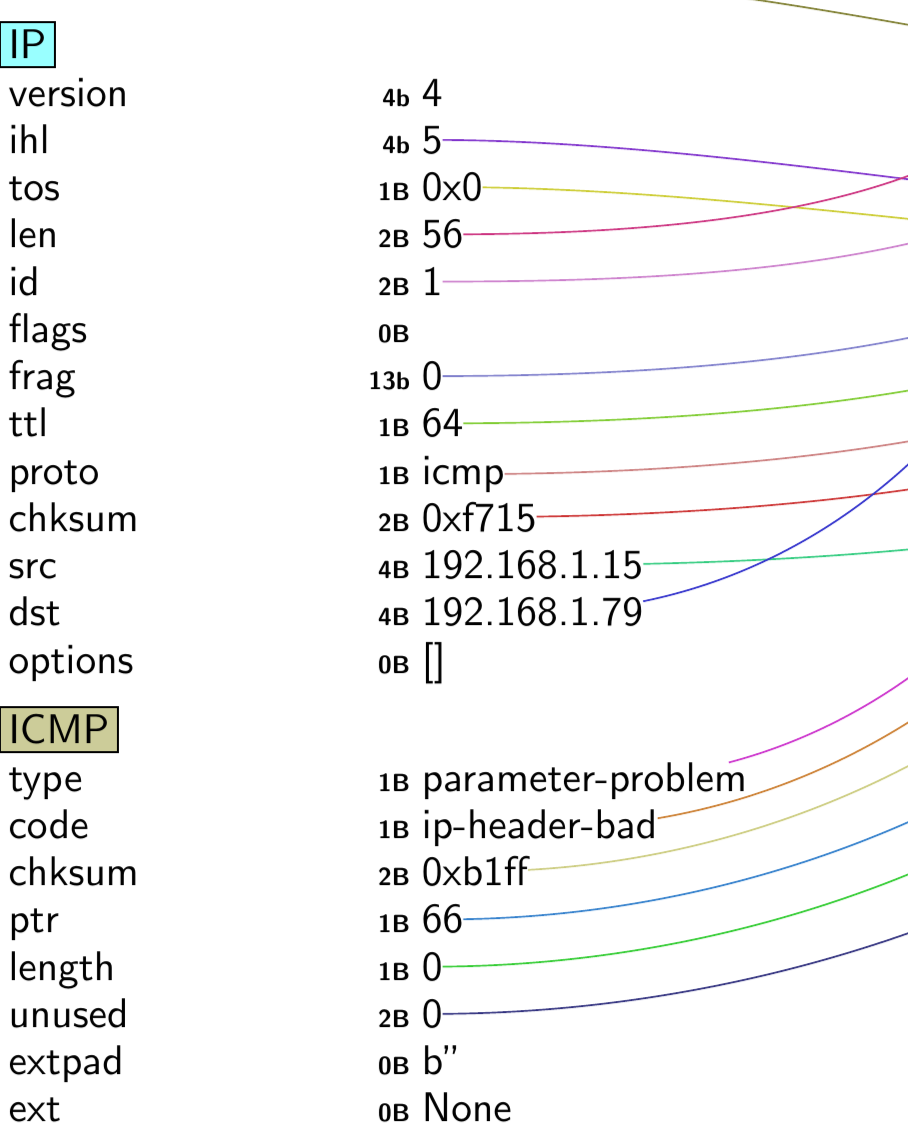
\includegraphics[width=0.5\textwidth]{./img/ICMP_storageCC/immagine_parameterproblem.png}
    \captionof{figure}{Messaggio IP/ICMP con campo \textit{unused} azzerato} 
    \label{fig:covertStorage:sourcequench:errScapy} 
\end{minipage}  
\vspace{2ex} \newline 
Il problema può essere risolto tramite degli accorgimenti.  
Tramite la libreria \textbf{struct} \cite{struct}, \uppercase{è} possibile 
inserire dei dati all'interno del campo. Infatti si può riscrivere, il 
pacchetto evitando di farlo creare Scapy. 
Così, quando lo si farà inviare da Scapy, al suo interno saranno presenti i dati. 
In Figura \ref{fig:covertStorage:unused} si vede la loro presenza. 
\newline
\begin{minipage}{\textwidth} 
    \centering
    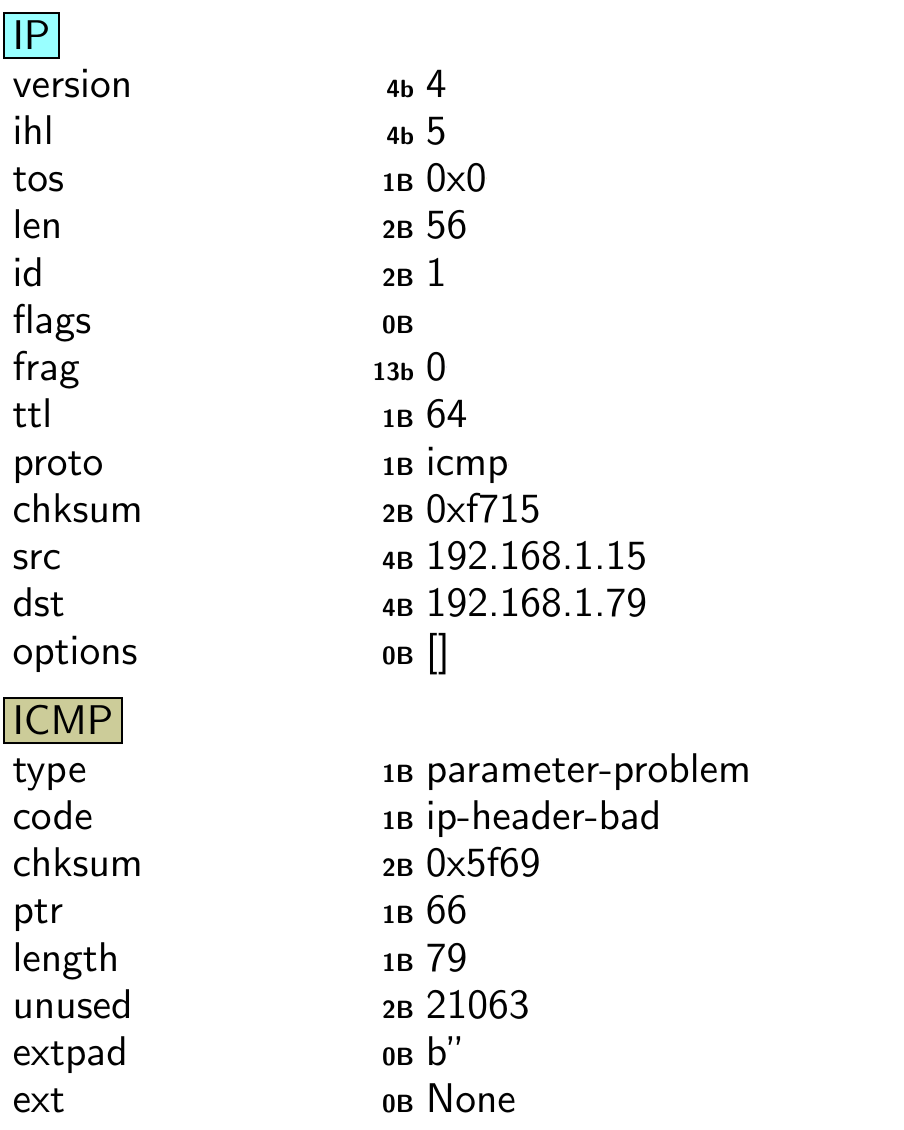
\includegraphics[width=0.5\textwidth]{./img/ICMP_storageCC/immagine_parameterproblem_unused.png}
    \captionof{figure}{Messaggio IP/ICMP con campo \textit{unused} impostato} 
    \label{fig:covertStorage:unused} 
\end{minipage} 
\vspace{2ex} \newline 
Siccome il suo utilizzo rende il messaggio non conforme agli standard RFC \cite{icmpv4_message_type}\cite{icmpv6_message_type}; 
un IDS che implementi la Deep Packet Inspection rileverà l'anomalia. 
Si potrà quindi scegliere se inserire dati nel campo o non. 
%Tuttavia nel nostro caso è stato utilizzato per testare la presenza della \textit{Deep Packet Inspection}.  

\subsubsection{Campo \textbf{Header+64 bits}} 
Nel campo si dovranno inserire l'header IP più 8 byte. %si potranno usare varie coppie nelle quali inserire i dati. 
Si potranno usare qindi varie tipologie di pacchetti purchè la loro lunghezza 
non superi i 28 byte.
\vspace{1ex} \newline
Inoltre siccome non rappresenta un datagram da inviare ma già spedito, 
si possono sfruttare un maggior numero di campi (indicati nella 
Tabella \ref{table:icmpv4:header64bit}). La Figura \ref{fig:covertStorage:header64bit}  
invece mostra un caso applicato ai protocolli IP e ICMP. 
\begin{longtable}{|p{0.3\textwidth}|p{0.3\textwidth}|p{0.3\textwidth}|} 
    \multicolumn{3}{c}{Header IPv4} \\  
    \hline 
    \textbf{Campo} & \textbf{Byte} & \textbf{Utilizzo} \\
    \hline 
    Time to live & 1 byte & Tempo di vita del pacchetto\\  
    \hline 
    Total length & 2 byte & Dimensione dell'intero pacchetto\\  
    \hline
    Identification & 2 byte & Identifica i frammenti di un pacchetto IP \\ 
    \hline 
    \noalign{\vskip 2ex}
    \multicolumn{3}{c}{Header ICMPv4} \\ 
    \hline
    \textbf{Campo} & \textbf{Byte} & \textbf{Utilizzo} \\
    \hline
    %Aiuta nell'accoppiare le richieste e le risposte
    Identifier & 2 byte & Identificativo del messaggio di richiesta invocato \\  
    \hline 
    Sequence & 2 byte & Numero di sequenza del messaggio di richiesta invocato \\  
    \hline
    \caption{Uso del Header+64 bits nel caso di IP/ICMP} 
    \label{table:icmpv4:header64bit} 
\end{longtable} 
%Ma può essere utilizzato anche TCP/IP o altri protocolli purchè lunghezza passata, 
%non sfori i 28 bytes.-
%si userà il campo \textbf{len} del protocollo \textit{IP} e il campo \textbf{id} del protocollo \textit{ICMP}. 
%Tuttavia si dovrebbe inserire solo il primo byte del datagram originale. 
%Ciò cambierà la visibilità del pacchetto siccome non conforme allo standard. 
\begin{minipage}{\textwidth}
    \centering
    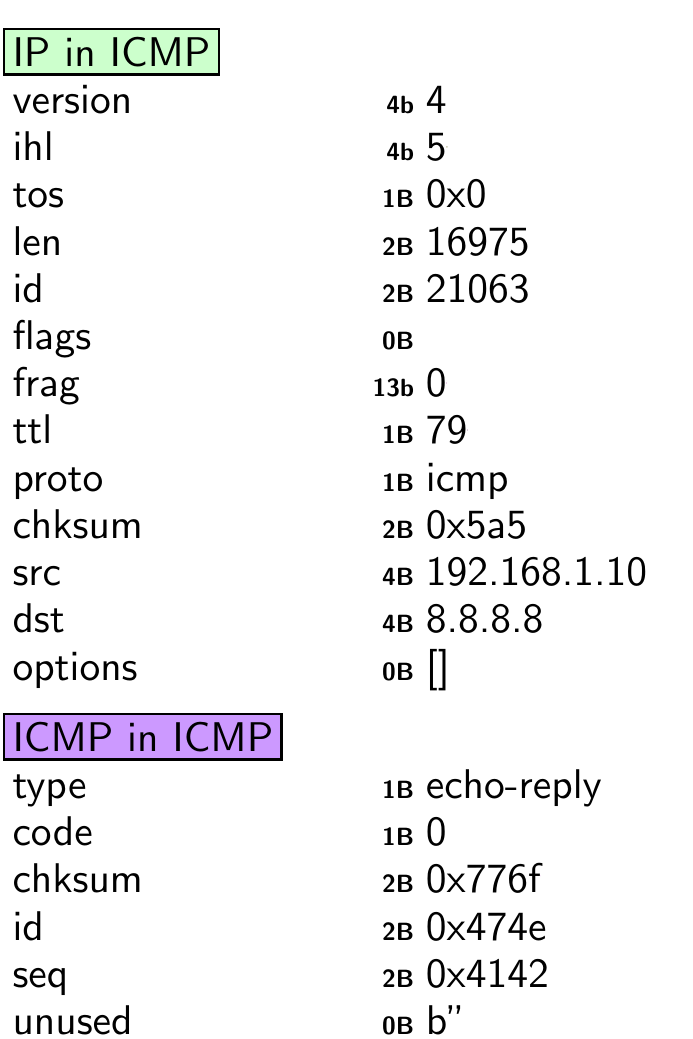
\includegraphics[width=0.5\textwidth]{./img/ICMP_storageCC/immagie_header_64bit.png}
    \captionof{figure}{Messaggio IP/ICMP con campo \textit{Header+64 bit} impostato} 
    \label{fig:covertStorage:header64bit} 
\end{minipage} 
\begin{center}
\begin{minipage}{0.9\linewidth}
\centering
\begin{lstlisting} [basicstyle=\ttfamily\scriptsize]
0000  24 77 03 18 7B 74 18 C0 4D 74 BB AE 08 00 45 00  $w..{t..Mt....E.
0010  00 38 00 01 00 00 40 01 F7 15 C0 A8 01 0F C0 A8  .8....@.........
0020  01 4F 03 03 68 66 42 4F 52 47 45 00 4F 47 4E 41  .O..hfBORGE.OGNA
0030  00 00 42 01 09 B3 C0 A8 01 0A 08 08 08 08 00 00  ..B.............
0040  69 5E 4F 52 47 4F                                i^ORGO
\end{lstlisting}
\captionof{lstlisting}{Dump esadecimale del messaggio in figura \ref{fig:covertStorage:header64bit}}
\label{code:covertStorage:header64bit} 
\end{minipage}
\end{center}

\subsubsection{Campo \textbf{Invoking Packet}} 
Quando si indicha il pacchetto che ha causato l'errore, si dovrà stare 
attenti a non superare la \textit{IPv6 MTU}. 
Nel nostro caso, ciò non succederà siccome si useranno i protocolli IPv4 la 
cui intestazione è di 40 byte, ed il protocollo ICMPv4, la cui intestazione 
è di 8 byte. 
%Nel campo \textbf{Invoking Packet} si userà il campo \textbf{plen} del protocollo \textit{IPv6} e il campo \textbf{id} del protocollo \textit{ICMPv6}. 
La Tabella \ref{table:icmpv6:invokinppacket} indica i campi utilizzati nel caso IPv6/ICMPv6. 
\newline
\begin{longtable}{|p{0.3\textwidth}|p{0.3\textwidth}|p{0.3\textwidth}|} 
    \multicolumn{3}{c}{Header IPv6} \\ 
    \hline 
    \textbf{Campo} & \textbf{Byte} & \textbf{Utilizzo} \\
    \hline 
    Payload Length & 2 byte & Tempo di vita del pacchetto\\  
    \hline 
    Hop Limit & 1 byte & Decrementato di 1 per ogni nodo che inoltra il pacchetto\\  
    \hline 
    \multicolumn{3}{c}{Header ICMPv6} \\
    \hline
    \textbf{Campo} & \textbf{Byte} & \textbf{Utilizzo} \\
    \hline
    Identifier & 2 byte & Identificativo del messaggio di richiesta invocato\\  
    \hline 
    Sequence & 2 byte & Numero di sequenza del messaggio di richiesta invocato \\  
    \hline 
    \caption{Struttura del campo Invoking Packet} 
    \label{table:icmpv6:invokinppacket} 
\end{longtable}


\subsubsection{Campo \textbf{Pointer}} 
Indica l'ottetto del messaggio in cui è presente l'errore; 
tuttavia può contenere dei dati non correlati ad esso. 
Nel nostro caso, verranno inseriti tanti dati quanto la sua capacità; 
come mostra la Figura \ref{fig:covertStorage:pointer}. 
%può contenere i dati e, siccome rappresenta l'ottetto in cui è stato rilevato l'errore, potrà essere variabile.
\newline 
\begin{minipage}{\textwidth}
    \centering
    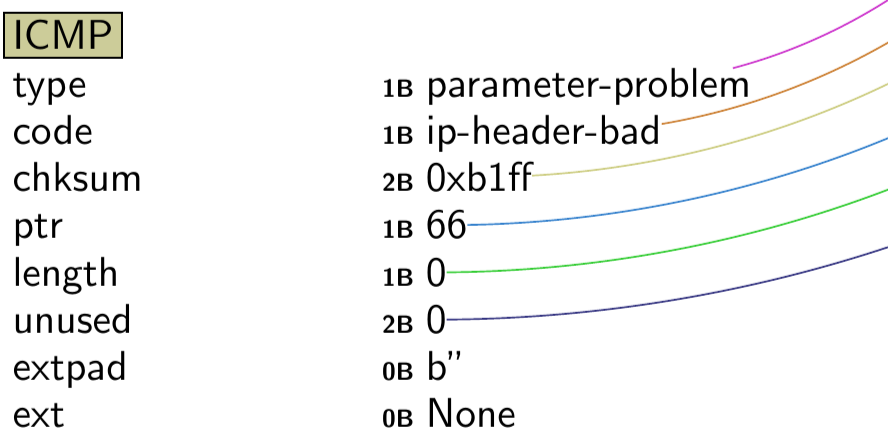
\includegraphics[width=0.6\textwidth]{./img/ICMP_storageCC/immagine_pointer.png}
    \captionof{figure}{Messaggio IP/ICMP con campo \textit{pointer} impostato} 
    \label{fig:covertStorage:pointer} 
\end{minipage} 
\begin{center}
\begin{minipage}{0.9\linewidth}
\centering
\begin{lstlisting} [basicstyle=\ttfamily\scriptsize]
0000  24 77 03 18 7B 74 18 C0 4D 74 BB AE 08 00 45 00  $w..{t..Mt....E.
0010  00 38 00 01 00 00 40 01 F7 15 C0 A8 01 0F C0 A8  .8....@.........
0020  01 4F 0C 00 B1 FF 42 00 00 00 45 00 4F 52 47 4F  .O....B...E.ORGO
0030  00 00 47 01 0B 9A C0 A8 01 0A 08 08 08 08 00 00  ..G.............
0040  6F 6F 4E 41 42 4F                                ooNABO
\end{lstlisting}
\captionof{lstlisting}{Dump esadecimale del messaggio in Figura \ref{fig:covertStorage:pointer}}
\label{code:covertStorage:pointer} 
\end{minipage}
\end{center}

\subsubsection{Campo \textbf{Identifier} e \textbf{Sequenza}}
Il campo \textit{Identifier} definisce l'identificativo delle richieste e 
può assumere un qualsiasi valore. 
Il campo \textit{Sequenza} (dalle specifiche RFC 792 \cite{icmpv4_message_type}), 
viene incrementato ad ogni richiesta inviata con lo stesso Identifier. 
Se suo valore cambiasse troppo spesso la cosa potrebbe risultare sospetta 
(a differenza del campo \textit{Identifier}). %in maniera estremamente variabile (e non fosse strettamente crescente)
Quindi sebbene può essere utilizzato per inserire le informazioni, si 
userà quasi esclusivamente il campo Identifier (come mostra la Figura \ref{fig:covertStorage:identifier}). 
\newline
\begin{minipage}{\textwidth} 
    \centering
    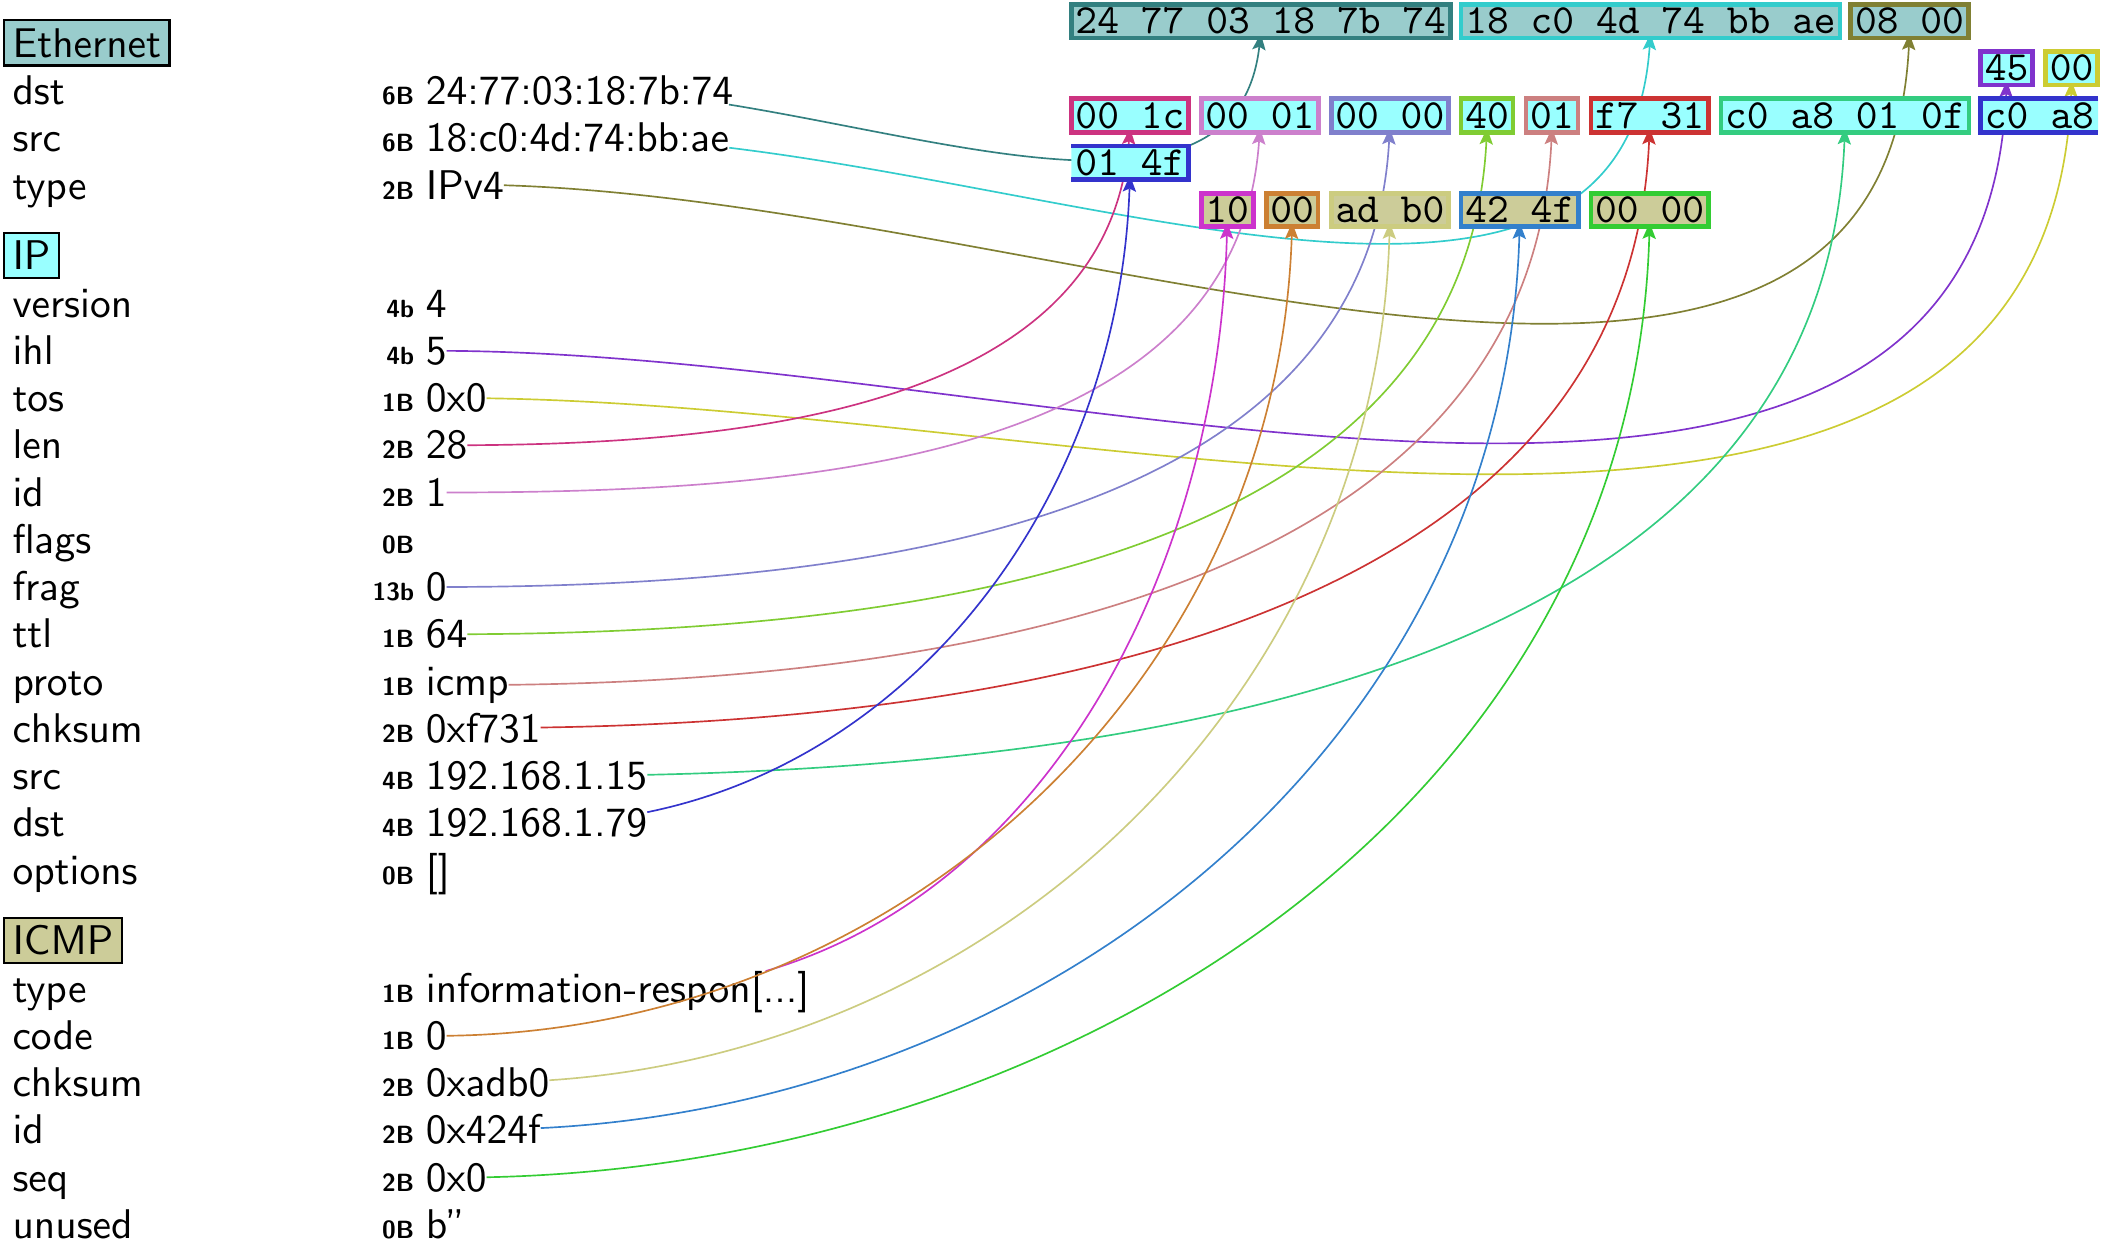
\includegraphics[width=\textwidth]{./img/ICMP_storageCC/imagine_identifier.png}
    \captionof{figure}{Messaggio IP/ICMP con campo \textit{identifier} impostato} 
    \label{fig:covertStorage:identifier} 
\end{minipage} 
\begin{center}
\begin{minipage}{0.9\linewidth}
\centering
\begin{lstlisting} [basicstyle=\ttfamily\scriptsize] 
#PACCHETTO No1
0000  24 77 03 18 7B 74 18 C0 4D 74 BB AE 08 00 45 00  $w..{t..Mt....E.
0010  00 1C 00 01 00 00 40 01 F7 31 C0 A8 01 0F C0 A8  ......@..1......
0020  01 4F 10 00 AD B0 42 4F 00 00                    .O....BO..

#PACCHETTO No2
0000  24 77 03 18 7B 74 18 C0 4D 74 BB AE 08 00 45 00  $w..{t..Mt....E.
0010  00 1C 00 01 00 00 40 01 F7 31 C0 A8 01 0F C0 A8  ......@..1......
0020  01 4F 10 00 9D B8 52 47 00 00                    .O....RG..

#PACCHETTO No3
0000  24 77 03 18 7B 74 18 C0 4D 74 BB AE 08 00 45 00  $w..{t..Mt....E.
0010  00 1C 00 01 00 00 40 01 F7 31 C0 A8 01 0F C0 A8  ......@..1......
0020  01 4F 10 00 A0 B8 4F 47 00 00                    .O....OG..

#PACCHETTO No4
0000  24 77 03 18 7B 74 18 C0 4D 74 BB AE 08 00 45 00  $w..{t..Mt....E.
0010  00 1C 00 01 00 00 40 01 F7 31 C0 A8 01 0F C0 A8  ......@..1......
0020  01 4F 10 00 A1 BE 4E 41 00 00                    .O....NA..
\end{lstlisting}
\captionof{lstlisting}{Dump esadecimale del messaggio in Figura \ref{fig:covertStorage:identifier}}
\label{code:covertStorage:identifier} 
\end{minipage}
\end{center}

\subsubsection{Campo \textbf{Data}} 
In questo campo il mittente può inserire quanti dati preferisce. 
Ma per sicurezza la dimensione sarà o 32 o 64 byte. 
Inoltre una quantità di dati eccessiva può far mandare più pacchetti di risposta 
nel caso si fosse inviata una richiesta. 
%dovrà inferiore a 1400 bytes se non 
%strettamente uguale o inferiore a 32 bytes. %(o 56 bytes nel caso li si mandi da Linux).
\vspace{2ex} \newline  
\begin{minipage}{\textwidth}
    \centering
    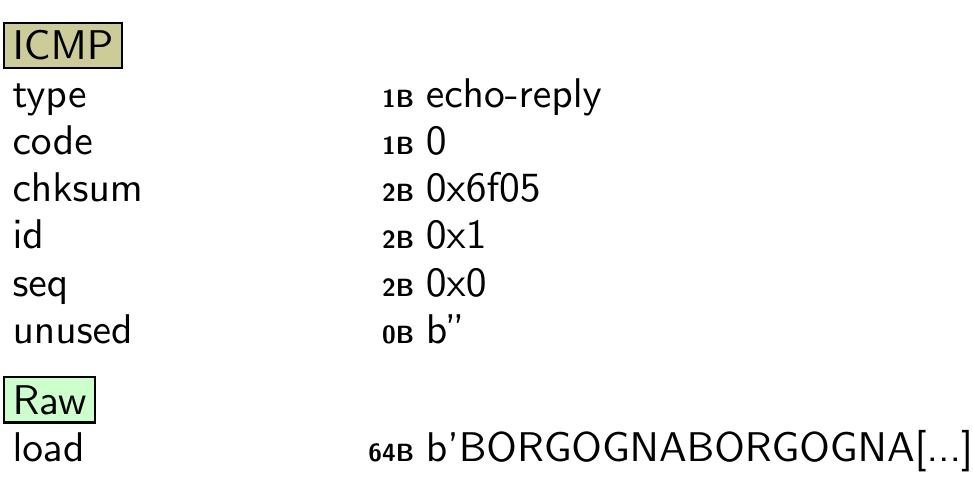
\includegraphics[width=0.7\textwidth]{./img/ICMP_storageCC/immagine_payload.png}
    \captionof{figure}{Messaggio IP/ICMP con campo \textit{Data} impostato} 
    \label{fig:covertStorage:payload} 
\end{minipage}  
\begin{center}
\begin{minipage}{0.9\linewidth}
\centering
\begin{lstlisting} [basicstyle=\ttfamily\scriptsize] 
0000  24 77 03 18 7B 74 18 C0 4D 74 BB AE 08 00 45 00  $w..{t..Mt....E.
0010  00 5C 00 01 00 00 40 01 F6 F1 C0 A8 01 0F C0 A8  .\....@.........
0020  01 4F 00 00 6F 05 00 01 00 00 42 4F 52 47 4F 47  .O..o.....BORGOG
0030  4E 41 42 4F 52 47 4F 47 4E 41 42 4F 52 47 4F 47  NABORGOGNABORGOG
0040  4E 41 42 4F 52 47 4F 47 4E 41 42 4F 52 47 4F 47  NABORGOGNABORGOG
0050  4E 41 42 4F 52 47 4F 47 4E 41 42 4F 52 47 4F 47  NABORGOGNABORGOG
0060  4E 41 42 4F 52 47 4F 47 4E 41                    NABORGOGNA
\end{lstlisting}
\captionof{lstlisting}{Dump esadecimale del messaggio in Figura \ref{fig:covertStorage:payload}}
\label{code:covertStorage:data} 
\end{minipage}
\end{center}

\subsubsection{Campo \textbf{Timestamp}}
Contiene i millisecondi dalla mezzanotte UT e ciascun campo ha un ordine temporale 
specifico; che dovrà rimanere congruente quando si inseriscono i dati. 
%Siccome i campi hanno un ordine temporale L'ordine dei tempi presenti in ciascuno dei campi dovrà essere congruente. 
%Si potrebbero inserire un numero magigore di dati sfruttando l'intera lunghezza dei campi ma 
%poi i tempi non risulterebbero congruenti fra di loro
%\footnote{Si potrebbe avere il caso che il destinatario ha modificato il messagio prima di poterlo ricevere}
Il Codice \ref{fig:covertStorage:timestamp:output} mostra come in ciascun 
campo timestamp verrà inserito un byte nella parte dei millisecondi. [Figura \ref{fig:covertStorage:timestamp:output}]. 
\newline
\begin{lstlisting}
Dato nascosto:  b'r'     114
Dato nascosto:  b'c'     99
Dato nascosto:  b'o'     111

Timestamp origin prima:  2025-11-07 23:13:36.146254+00:00
Timestamp origin dopo:  2025-11-07 23:13:36.114000+00:00
Tempo del campo:  83616114 
\end{lstlisting}
\captionof{lstlisting}{Esempio di un dato inserito nel campo Timestamp}
\label{fig:covertStorage:timestamp:output} 
\vspace{2ex} 
Non è possibile inserire ulteriori informazioni nelle altre parti  del 
campo temporale: rappresentando le ore, i minuti ed i secondi. 
Infatti hanno dei valori definiti e limitati, come si vede dalla Figura \ref{fig:covertStorage:time} (che mostra il valore contenuto nei campi). 
\vspace{1ex} \newline
Si potrebbero inserire il dato in tutto il campo rappresentnate il dato temporale; 
ma questo ci espone al rischio di avere tempi errati 
\footnote{
    Per esempio l pacchetto viene risultare ricevuto prima che sia stato inviato. 
}. 
\vspace{2ex} \newline 
Inoltre dalla Figura \ref{fig:covertStorage:time} si può constatare la presenza 
dell'informazione nella parte dei millisecondi. Dalle informazioni del pacchetto, 
i caratteri ricavati saranno le lettere R, G ed O; siccome i corrispettivi 
valori nella codifica ASCII \cite{ascii-table} sono 82, 71 e 79. 
\newline 
\begin{minipage}{\textwidth}
    \centering
    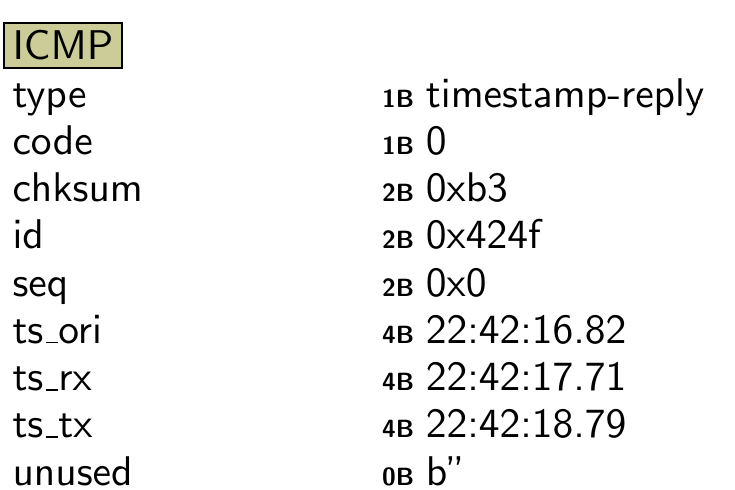
\includegraphics[width=0.6\textwidth]{./img/ICMP_storageCC/immagine_timestamp.png}
    \captionof{figure}{Messaggio IP/ICMP con campi \textit{Timestamp} impostati} 
    \label{fig:covertStorage:time} 
\end{minipage}   
\begin{center}
\begin{minipage}{0.9\linewidth}
\centering
\begin{lstlisting} [basicstyle=\ttfamily\scriptsize] 
#PACCHETTO No1
0000  24 77 03 18 7B 74 18 C0 4D 74 BB AE 08 00 45 00  $w..{t..Mt....E.
0010  00 28 00 01 00 00 40 01 F7 25 C0 A8 01 0F C0 A8  .(....@..%......
0020  01 4F 0E 00 00 B3 42 4F 00 00 04 DF 31 92 04 DF  .O....BO....1...
0030  35 6F 04 DF 39 5F                                5o..9_ 
#PACCHETTO No2
0000  24 77 03 18 7B 74 18 C0 4D 74 BB AE 08 00 45 00  $w..{t..Mt....E.
0010  00 28 00 01 00 00 40 01 F7 25 C0 A8 01 0F C0 A8  .(....@..%......
0020  01 4F 0E 00 FB C9 47 4E 00 00 04 DF 31 81 04 DF  .O....GN....1...
0030  35 6A 04 DF 39 5F                                5j..9_
\end{lstlisting}
\captionof{lstlisting}{Dump esadecimale del messaggio in Figura \ref{fig:covertStorage:time}}
\label{code:covertStorage:data} 
\end{minipage}
\end{center}

\subsubsection{Campo \textbf{MTU}}
Nel campo viene indicata la capacità massima del collegamento, 
Siccome il suo valore non è un valore prestabilito (ed è un intero 
variabile); l'intera dimensione del campo, potrà essere usato per inserire 
i dati. 